\chapter{Conjuntos de Dados}
\label{cap:conjuntos_de_dados}

Para realizar os experimentos deste estudo foi necessário dispor de conjuntos de dados amostrados através de sensores de abordagem passiva, aplicados em variações contextuais relacionadas aos fatores de dependência. Sendo assim, inicialmente realizamos o levantamento das principais bases de dados utilizadas em estudos envolvendo aplicações de ITS. Baseando-se em revisões anteriores \cite{Geyer2020}, elencamos características necessárias para condução dos experimentos e avaliamos a aderência a elas dos conjuntos de dados disponíveis. Embora os conjuntos possuam outros sensores, nossa análise focou a abordagem passiva.

Na \autoref{tabela:datasets} é detalhada a comparação. São utilizados os marcadores \emph{Sim (S)}, \emph{Não (N)} e \emph{Indefinido (I)}. São considerados \emph{S} os conjuntos que cumprem todos os requisitos de determinada característica, \emph{N} aqueles que não cumprem ao menos uma restrição, e \emph{I} quando não foi possível identificar informações do parâmetro avaliado. Na avaliação dos sensores inerciais e magnetômetro, foi considerado como requisito os conjuntos possuírem dados brutos nos três eixos. Para diferentes veículos, o requisito foi de utilizar diferentes modelos. Para ambientes, considerou-se diferentes superfícies, com variação de pavimentações ou não pavimentação. Para colocações, o requisito torna necessário ao menos um conjunto de sensores inerciais abaixo da suspensão e um acima. Por fim, o posicionamento controlado é requerido por produzir dados de forma mais confiável e permitir análises de propriocepção e exterocepção.

\begin{table}[h!]
    \small
    \centering
    \caption{Comparação de conjuntos de dados públicos}
    \label{tabela:datasets}
    \begin{tabular}{llcccccc}
\cmidrule(l){3-8}
 &  & \multicolumn{6}{c}{\textbf{Conjunto de Dados}} \\ \cmidrule(l){3-8} 
 & \textbf{} 
 & \textit{\href{http://www.cvlibs.net/datasets/kitti/setup.php}{KITTI}} 
 & \textit{\href{http://apolloscape.auto/index.html}{Apollo Scape}} 
 & \textit{\href{https://www.nuscenes.org/}{nuScenes}} 
 & \textit{\href{https://self-driving.lyft.com/level5/data/}{Lyft Level 5}} 
 & \textit{\href{https://waymo.com/open/}{Waymo}} 
 & \textit{\href{https://www.a2d2.audi/a2d2/en.html}{A2D2}} \\ \midrule
\multirow{5}{*}{\rotatebox[origin=c]{90}{\textbf{Sensores}}} & \textit{Câmera} & S & S & S & S & S & S \\ \cmidrule(l){2-8} 
 & \textit{GPS} & S & S & S & N & N & S \\ \cmidrule(l){2-8} 
 & \textit{Acelerômetro 3D} & S & S & N & N & N & S \\ \cmidrule(l){2-8} 
 & \textit{Giroscópio 3D} & S & S & S & N & N & N \\ \cmidrule(l){2-8} 
 & \textit{Magnetômetro 3D} & N & N & N & N & N & N \\ \midrule
\multirow{5}{*}{\rotatebox[origin=c]{90}{\textbf{Contexto}}} & \textit{Diferentes Veículos} & N & I & N & I & I & I \\ \cmidrule(l){2-8} 
 & \textit{Diferentes Condutores} & I & I & I & I & I & I \\ \cmidrule(l){2-8} 
 & \textit{Diferentes Ambientes} & I & I & I & I & I & I \\ \cmidrule(l){2-8} 
 & \textit{Diferentes Colocações} & N & N & N & N & N & N \\ \cmidrule(l){2-8} 
 & \textit{Posicionamento Controlado} & S & I & S & N & N & I \\ \bottomrule
\end{tabular}
    \fonte{Desenvolvido pelo autor.}
\end{table}

Conforme observado na análise comparativa, nenhum dos conjuntos de dados disponíveis apresenta dados para todos os sensores necessários, dentre sensores inerciais e de suporte. Na análise de contexto as características avaliadas se mostram ainda menos presentes, especialmente por conta de os sensores inerciais não serem o foco de nenhum dos conjuntos e, portanto, sua abordagem de coleta não ser tratada de forma adequada. Em geral, as propriedades avaliadas como \emph{I} são propensas a serem \emph{N}, uma vez que sua não especificação tende a ter sido em razão de não ser considerada ou não existir. Em uma análise ampla, nenhum dos conjuntos de dados avaliados atende os requisitos para experimentação deste estudo e, por isso, se fez necessário conduzir uma etapa de coleta de dados, detalhada nas próximas subseções.

\section{Rede de Sensores}

Para coletar os dados foram desenvolvidas duas redes de sensores, sendo cada uma delas composta por um SBC Raspberry Pi e três módulos MPU-9250, cada um deles equipado com um acelerômetro 3D, giroscópio 3D, magnetômetro 3D e um sensor de temperatura. Uma fonte externa de GPS também foi utilizada, produzindo dados de localização e velocidade, assim como uma câmera para captura de vídeo do ambiente. A \autoref{tabela:rede_de_sensores} detalha o \textit{hardware} utilizado.

\begin{table}[h!]
\small
\caption{Hardware da rede de sensores} 
\label{tabela:rede_de_sensores}
\centering
\begin{tabular}{llll}
\toprule
\multicolumn{1}{l}{\textbf{Hardware}} & 
\multicolumn{1}{l}{\textbf{Sensor}} & 
\multicolumn{1}{l}{\textbf{Dados}} & 
\multicolumn{1}{l}{\textbf{Taxa}}  
\\ \midrule

\multicolumn{1}{l}{HP Webcam HD-4110} & 
\multicolumn{1}{l}{Câmera} & 
\multicolumn{1}{l}{Vídeo 720p} & 
\multicolumn{1}{c}{30 Hz}                   
\\ \midrule

\multicolumn{1}{l}{Xiaomi Mi 8} & 
\multicolumn{1}{l}{GPS} & 
\multicolumn{1}{l}{Velocidade em $m/s$, latitude, longitude, etc.} &
\multicolumn{1}{c}{1 Hz}
\\ \midrule

\multicolumn{1}{l}{\multirow{5}{*}{MPU-9250}} & 
\multicolumn{1}{l}{Acelerômetro} & 
\multicolumn{1}{l}{Aceleração 3D em $m/s^2$} &
\multicolumn{1}{c}{\multirow{5}{*}{100 Hz}} 
\\ \cmidrule(lr){2-3}

\multicolumn{1}{l}{} & 
\multicolumn{1}{l}{Giroscópio} & 
\multicolumn{1}{l}{Taxa de rotação 3D em $graus/s$} & 
\multicolumn{1}{l}{}                       
\\ \cmidrule(lr){2-3}

\multicolumn{1}{l}{} & 
\multicolumn{1}{l}{Magnetômetro} & 
\multicolumn{1}{l}{Campo geomagnético ambiente 3D em $\mu T$} & 
\multicolumn{1}{l}{}
\\ \cmidrule(lr){2-3}

\multicolumn{1}{l}{} & 
\multicolumn{1}{l}{Temperatura} &
\multicolumn{1}{l}{Temperatura em $^{\circ}C$} & 
\multicolumn{1}{l}{}                       
\\ \bottomrule

\end{tabular}
\fonte{Desenvolvido pelo autor.}
\end{table}

Todo o equipamento foi fixado no veículo conforme detalha a \autoref{fig:colocacao_posicionamento_rede_sensores}. A câmera foi colocada na parte externa do teto do carro (1), capturando vídeo do ambiente em 30Hz. O receptor GPS foi colocado internamente no painel (2), amostrando dados em 1Hz. Os seis módulos MPU-9250 foram distribuídos no veículo de forma a considerar os dados provindos de pontos com diferentes influências da propriedade de dependência veicular. Sendo assim, em ambas as extremidades do eixo dianteiro (lado direito e esquerdo) foi anexado um módulo ao braço de controle (4), localizado abaixo e próximo à suspensão do veículo; outro módulo foi colocado acima e próximo da suspensão, anexado à carroceria imediatamente acima do pneu (3); e outro módulo foi anexado no painel do veículo (2), dentro da cabine. Em relação ao referencial de amostragem dos módulos MPU-9250, foi utilizada a abordagem de posicionamento controlado, onde a colocação dos módulos foi realizada de forma que os três eixos do sistema de coordenadas do sensor ficaram alinhados com os do veículo, sendo tanto referencial de coleta como de análise. O acelerômetro foi ajustado em um \textit{Full Scale Range} (FSR) de 8$g$ e o giroscópio de 1000$graus/s$, constituindo intervalos consistentes para não saturar, ambos amostrando em 100Hz (propriedades sensoriais).

\begin{figure}[h!]
  \centering
  \caption{Colocação e posicionamento da rede de sensores no veículo}
   \label{fig:colocacao_posicionamento_rede_sensores}
   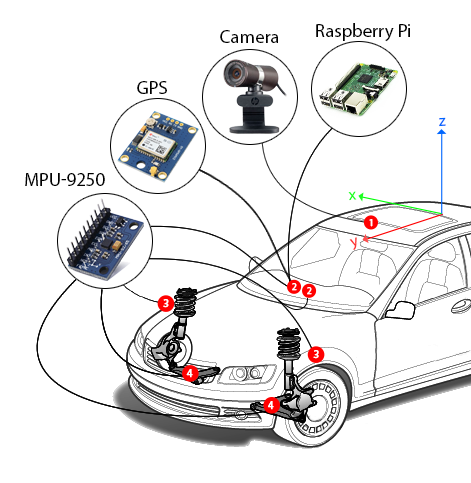
\includegraphics[width=0.69\textwidth]{figuras/fig_22.png}
   \fonte{Desenvolvido pelo autor.}
\end{figure}

\section{Execução da Coleta}

Para o desenvolvimento e validação de modelos de percepção veicular adaptativa, se mostrou necessário produzir dados em variações contextuais para obter variabilidade de condições relacionadas aos fatores de dependência. Sendo assim, além da amostragem de velocidade (propriedade de condução) e da colocação dos sensores inerciais em diferentes pontos da estrutura veicular (propriedade veicular), nós realizamos diversas coletas de dados utilizando da rede de sensores em três diferentes modelos de veículos (propriedade veicular), com três diferentes motoristas variando a velocidade de 0 \emph{km/h} até 91,98 \emph{km/h} (propriedade de condução) trafegando em três cenários distintos (propriedade ambiental). Cada cenário contém vias sem pavimentação (terra) e trechos pavimentados (asfalto ou paralelepípedo), com variações gerais do ambiente, tais como presença de lombadas, buracos, diferentes níveis de conservação do pavimento, etc. Detalhes dos cenários são apresentados na próxima seção. Sendo assim, foram produzidos nove conjuntos de dados denominados \textit{Passive Vehicular Sensors Dataset} (PVS 1-9), detalhados na \autoref{table:descricao_conjuntos}. Cada um dos conjuntos de dados é composto pelos arquivos especificados na \autoref{table:conjuntos_arquivos}. Os dados foram coletados no município de Anita Garibaldi, no interior do estado de Santa Catarina, Brasil, entre os dias 24 e 26 de dezembro de 2019. O ponto médio dos cenários é dado pelas coordenadas (-27,69983094872972, -51,11577673365139).

\begin{table}[H]
\small
\caption{Conjuntos de dados produzidos} 
\label{table:descricao_conjuntos}
\centering
\begin{tabular}{llll}
\toprule
\textbf{Nome} & \textbf{Veículo} & \textbf{Condutor} & \textbf{Cenário} \\ \midrule
PVS 1 & Volkswagen Saveiro & Condutor 1 & Cenário 1 \\ \midrule
PVS 2 & Volkswagen Saveiro & Condutor 1 & Cenário 2 \\ \midrule
PVS 3 & Volkswagen Saveiro & Condutor 1 & Cenário 3 \\ \midrule
PVS 4 & Fiat Bravo & Condutor 2 & Cenário 1 \\ \midrule
PVS 5 & Fiat Bravo & Condutor 2 & Cenário 2 \\ \midrule
PVS 6 & Fiat Bravo & Condutor 2 & Cenário 3 \\ \midrule
PVS 7 & Fiat Palio & Condutor 3 & Cenário 1 \\ \midrule
PVS 8 & Fiat Palio & Condutor 3 & Cenário 2 \\ \midrule
PVS 9 & Fiat Palio & Condutor 3 & Cenário 3 \\ \bottomrule
\end{tabular}
\fonte{Desenvolvido pelo autor.}
\end{table}

\vspace{-1.1cm}

\begin{table}[H]
\small
\caption{Arquivos que compõe cada conjunto de dados} 
\label{table:conjuntos_arquivos}
\centering
\begin{tabular}{ll}
\toprule
\textbf{Arquivo} & \textbf{Descrição} \\ \midrule
dataset\_gps.csv & Dados de GPS, incluindo latitude, longitude, altitude, velocidade, \\ & acurácia, etc. \\ \midrule
dataset\_gps\_mpu\_left.csv & Dados dos MPUs colocados no lado esquerdo do veículo, \\ & combinados com dados GPS. \\ \midrule
dataset\_gps\_mpu\_right.csv & Dados dos MPUs colocados no lado direito do veículo, \\ & combinados com dados GPS. \\ \midrule
dataset\_labels.csv & Classes de dados para cada amostra do conjunto de dados \\ & (para ambos os lados). \\ \midrule
dataset\_mpu\_left.csv & Dados dos MPUs colocados no lado esquerdo do veículo. \\ \midrule
dataset\_mpu\_right.csv & Dados dos MPUs colocados no lado direito do veículo. \\ \midrule
dataset\_settings\_left.csv & Configurações dos MPUs colocados no lado esquerdo \\ & do veículo. Inclui faixa de medição, resolução, etc. \\ \midrule
dataset\_settings\_right.csv & Configurações dos MPUs colocados no lado direito \\ & do veículo. Inclui faixa de medição, resolução, etc. \\ \midrule
map.html & Mapas interativos com os dados e as classes. \\ \midrule
video\_dataset\_left.mp4 & Vídeo com gráficos dos dados dos MPUs e GPS, amostrados \\ & no lado esquerdo do veículo. \\ \midrule
video\_dataset\_right.mp4 & Vídeo com gráficos dos dados dos MPUs e GPS, amostrados \\ & no lado direito do veículo. \\ \midrule
video\_environment.mp4 & Vídeo do ambiente externo. \\ \midrule
video\_environment\_dataset\_left.mp4 & Vídeos lado a lado de video\_environment.mp4 e \\ & video\_dataset\_left.mp4 \\ \midrule
video\_environment\_dataset\_right.mp4 & Vídeos lado a lado de video\_environment.mp4 e \\ & video\_dataset\_right.mp4 \\ \bottomrule
\end{tabular}
\fonte{Desenvolvido pelo autor.}
\end{table}

\section{Classes de Dados}

Para criação dos rótulos correspondentes às classes de dados, foram utilizados GT de anotação humana e de anotação automatizada por máquina. Os primeiros rótulos criados foram os das classes de dados de tipo de superfície de pista. Para essas classes, foram criados os rótulos \emph{terra} (\texttt{dirt\_road}), \emph{paralelepípedo} (\texttt{cobblestone\_road}) e \emph{asfalto} (\texttt{asphalt\_road}). A anotação foi realizada via GT humano, uma vez que esta classe representa uma característica objetiva. Desta forma, através da observação do que a roda toca por meio do vídeo capturado, os delimitadores de início e fim dessas classes puderam ser facilmente apontados. A \autoref{fig:tipos_superficie} ilustra os tipos de superfície presentes em todos os conjuntos de dados PVS, com a \autoref{fig:mapa_superficies} detalhando a distribuição delas no mapa de cada cenário. A \autoref{table:tipos_superficie_metricas} detalha as métricas para cada conjunto, com a quantificação das amostras e a proporção da distribuição das classes de dados, informações importantes para se analisar o nível de desbalanceamento das classes antes do treinamento dos modelos. 

\begin{figure}[H]
  \centering
  \caption{Tipos de superfície presentes nos cenários}
   \label{fig:tipos_superficie}
   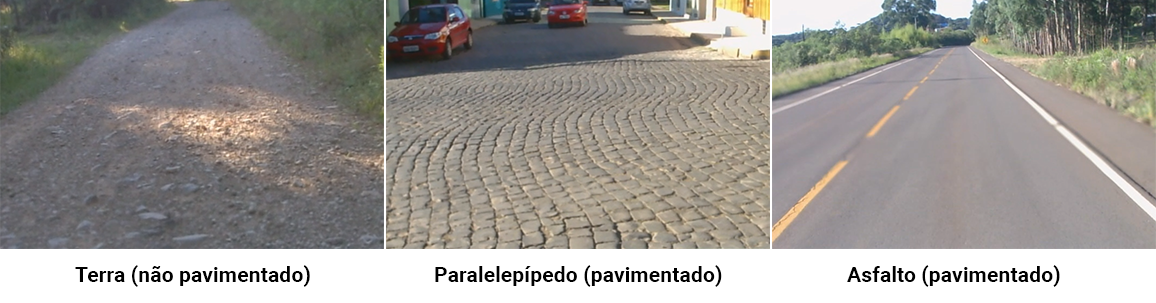
\includegraphics[width=1\textwidth]{figuras/fig_23.png}
   \fonte{Desenvolvido pelo autor.}
\end{figure}

\begin{figure}[H]
  \centering
  \caption{Mapa das superfícies presentes nos cenários.}
   \label{fig:mapa_superficies}
   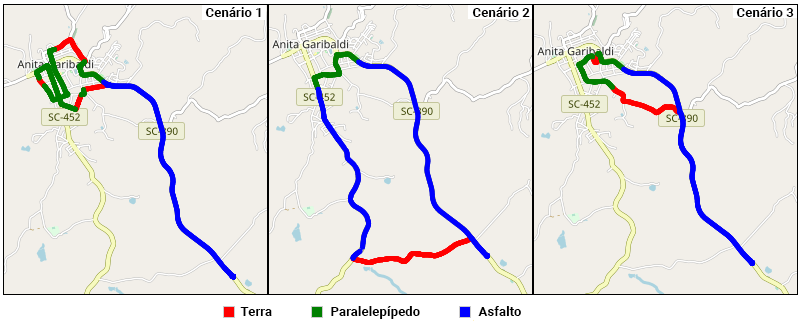
\includegraphics[width=1\textwidth]{figuras/fig_25.png}
   \fonte{Desenvolvido pelo autor.}
\end{figure}

\begin{table}[H]
\scriptsize
\centering
\caption{Quantificação para as classes de dados de tipo de superfície} 
\label{table:tipos_superficie_metricas}
\begin{tabular}{ccccccccc}
\cmidrule(l){3-9} & & 
\multicolumn{4}{c}{\textbf{Número de Amostras}} & 
\multicolumn{3}{c}{\textbf{Distribuição das Classes de Dados (\%)}} 
\\ \midrule

\multicolumn{1}{c}{\textbf{Cenário}} &
\textbf{Conjunto} &
\textbf{Terra} &
\textbf{Paralelepípedo} &
\textbf{Asfalto} & 
\textbf{Total} &
\textbf{Terra} &
\textbf{Paralelepípedo} &
\textbf{Asfalto}
\\ \midrule

\multicolumn{1}{c}{\multirow{4}{*}{1}} & PVS 1 & 25868 & 61659 & 56509 & 144036 & 17,96 & 42,81 & 39,23 \\ \cmidrule(l){2-9} 
\multicolumn{1}{c}{} & PVS 4 & 23903 & 57670 & 50919 & 132492 & 18,04 & 43,53 & 38,43 \\ \cmidrule(l){2-9} 
\multicolumn{1}{c}{} & PVS 7 & 23778 & 54224 & 50546 & 128548 & 18,50 & 42,18 & 39,32 \\ \midrule

\multicolumn{1}{c}{\multirow{4}{*}{2}} & PVS 2 & 44618 & 20737 & 59330 & 124685 & 35,78 & 16,63 & 47,58 \\ \cmidrule(l){2-9} 
\multicolumn{1}{c}{} & PVS 5 & 60539 & 18143 & 55195 & 133877 & 45,22 & 13,55 & 41,23 \\ \cmidrule(l){2-9} 
\multicolumn{1}{c}{} & PVS 8 & 44939 & 18825 & 59854 & 123618 & 36,35 & 15,23 & 48,42 \\ \midrule

\multicolumn{1}{c}{\multirow{4}{*}{3}} & PVS 3 & 28659 & 26143 & 51014 & 105816 & 27,08 & 24,71 & 48,21 \\ \cmidrule(l){2-9} 
\multicolumn{1}{c}{} & PVS 6 & 23888 & 31641 & 40750 & 96279 & 24,81 & 32,86 & 42,32 \\ \cmidrule(l){2-9} 
\multicolumn{1}{c}{} & PVS 9 & 23153 & 25182 & 43220 & 91555 & 25,29 & 27,50 & 47,21 \\ \bottomrule

\end{tabular}
\fonte{Desenvolvido pelo autor,}
\end{table}

O segundo grupo de classes de dados rotuladas foi o de lombadas. Assim como as classes de tipo de superfície, as de lombadas correspondem a características objetivas e foram anotadas com GT humano. Foram criados os rótulos \emph{com lombada} (\texttt{asphalt\_speed\_bump} e \texttt{cobblestonne\_speed\_bump}), e \emph{sem lombada} (\texttt{no\_speed\_bump}). As lombadas foram amostradas nos dois tipos de pavimentação, conforme ilustra a \autoref{fig:lombadas_superficies}. A \autoref{fig:lombadas_mapa} detalha as localizações das lombadas, e a \autoref{table:lombada_metricas} especifica as métricas destas classes de dados.

\begin{figure}[h!]
  \centering
  \caption{Lombadas em diferentes superfícies presentes nos cenários}
   \label{fig:lombadas_superficies}
   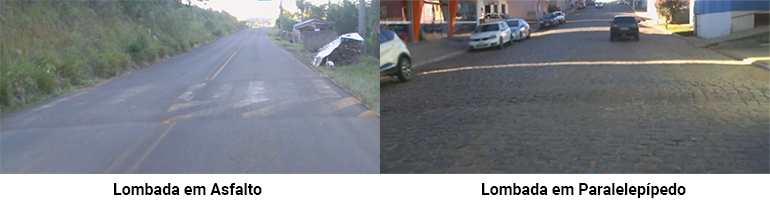
\includegraphics[width=0.85\textwidth]{figuras/fig_24.png}
   \fonte{Desenvolvido pelo autor.}
\end{figure}

\begin{figure}[h!]
  \centering
  \caption{Lombadas em diferentes superfícies presentes nos cenários}
   \label{fig:lombadas_mapa}
   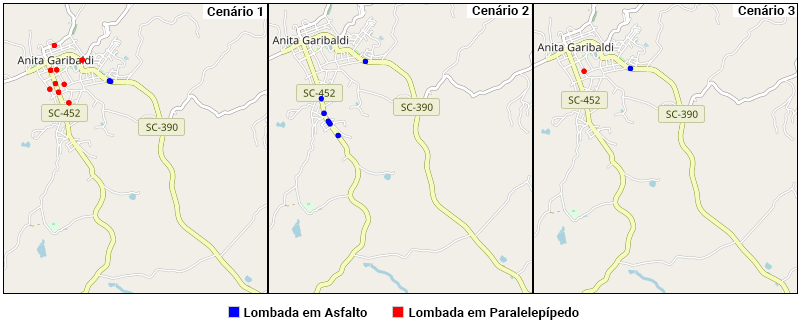
\includegraphics[width=1\textwidth]{figuras/fig_26.png}
   \fonte{Desenvolvido pelo autor.}
\end{figure}

\begin{table}[H]
\scriptsize
\centering
\caption{Quantificação para as classes de dados de lombadas} 
\label{table:lombada_metricas}
\begin{tabular}{ccccccc}
\cmidrule(l){3-7}
\multicolumn{1}{l}{} & 
\multicolumn{1}{l}{} & 
\multicolumn{3}{c}{\textbf{Número de Amostras}} & 
\multicolumn{2}{c}{\textbf{Distribuição das Classes de Dados (\%)}} \\ \midrule
\textbf{Cenário} & 
\textbf{Conjunto} & 
\textbf{Com Lombada} & 
\textbf{Sem Lombada} & 
\textbf{Total} & 
\textbf{Com Lombada} & 
\textbf{Sem Lombada} \\ \midrule

\multirow{4}{*}{1} & PVS 1 & 3455 & 140581 & 144036 & 2,39 & 97,60 \\ \cmidrule(l){2-7} 
 & PVS 4 & 3134 & 129358 & 132492 & 2,37 & 97,63 \\ \cmidrule(l){2-7} 
 & PVS 7 & 2876 & 125672 & 128548 & 2,24 & 97,76 \\ \midrule
 
\multirow{4}{*}{2} & PVS 2 & 2006 & 122679 & 124685 & 1,61 & 98,39 \\ \cmidrule(l){2-7} 
 & PVS 5 & 1943 & 131934 & 133877 & 1,45 & 98,55 \\ \cmidrule(l){2-7} 
 & PVS 8 & 1837 & 121781 & 123618 & 1,49 & 98,51 \\ \midrule
 
\multirow{4}{*}{3} & PVS 3 & 609 & 105207 & 105816 & 0,57 & 99,42 \\ \cmidrule(l){2-7} 
 & PVS 6 & 606 & 95673 & 96279 & 0,63 & 99,37 \\ \cmidrule(l){2-7} 
 & PVS 9 & 643 & 90914 & 91557 & 0,71 & 99,30 \\ \bottomrule
\end{tabular}
\fonte{Desenvolvido pelo autor,}
\end{table}

Por fim, foram criados os rótulos para o nível de qualidade da superfície de pista. Para estas classes de dados, foram criados os rótulos \emph{boa} (\texttt{good\_road}), \emph{regular} (\texttt{regular\_road}) e \emph{ruim} (\texttt{bad\_road}). Ao contrário das classes anteriores, as classes de qualidade podem tornar-se subjetivas de acordo com o GT utilizado. Inúmeros estudos rotulam a qualidade com base na percepção de qualidade de um usuário ou através da quantificação de irregularidades e obstáculos presentes no segmento de pista. Contudo, utilizar GT de anotação humana através das metodologias descritas acima torna as classes subjetivas, com viés a percepção de quem rotulou. Logo, de forma a tratar este problema, desenvolvemos um GT de anotação automatizada por máquina, baseado na análise de vibração.

O processo de anotação de qualidade de superfície se inicia com a quantificação da irregularidade longitudinal dos segmentos analisados, baseado no cálculo de IRI de \cite{Li2018}. A irregularidade calculada corresponde ao conjunto de desvios da superfície em relação a um plano de referência. Sendo assim, partindo de um \textit{baseline} onde a variação dos sinais dos sensores inerciais é 0, caracterizando um segmento regular, quanto maior essa variação (vibração), mais irregular é a superfície. Para calcular a irregularidade, foi empregado RMS, a qual consiste de uma técnica estatística que mede a magnitude de uma variação, sendo especialmente útil quando os valores empregados alternam entre positivos e negativos, como é o caso dos sinais analisados. 

A utilização do RMS com os dados dos sensores inerciais fornece a magnitude da irregularidade da superfície com a influência dos fatores de dependência. Sendo assim, é necessário considerar a forma com que cada um dos fatores influencia o valor resultante. Desta forma, após seu cálculo, a magnitude da irregularidade (propriedade ambiental) é normalizada pela velocidade acumulada no segmento de dados (propriedade de condução) \cite{Li2018}. Em suma, nesta primeira etapa, através de uma janela deslizante de 500 amostras, com 250 amostras à direita e outras 250 à esquerda, os sinais são convolvidos aplicando sobre eles RMS normalizado pela velocidade acumulada no segmento. A equação abaixo detalha este cálculo, onde \emph{i} é o índice da primeira amostra da janela, \emph{j} o índice da última amostra, \emph{R} o RMS dos sinais dos sensores inerciais, e \emph{v} a velocidade.

\begin{center}
  \[
  \textit{Vibração} = \frac{(j - i + 1) \cdot R}{\sum_{x=i}^{j} v_x} \cdot 100
  \]
\end{center}

As características de vibração foram extraídas para cada um dos conjuntos PVS. Em seguida, estas características foram agrupadas de acordo com o modelo de veículo utilizado (propriedade veicular), onde no primeiro grupo ficaram as características dos PVS 1-3 (Volkswagen Saveiro), no segundo as dos PVS 4-6 (Fiat Bravo), e no terceiro as dos PVS 7-9 (Fiat Palio). Uma vez que os três cenários de coleta de dados contam com ambientes nos quais há segmentos nos três níveis de qualidade, e que cada um dos agrupamentos por veículo conta com dados dos três cenários, podemos concluir que necessariamente cada agrupamento possui características de alto nível que representam segmentos com pista de qualidade boa, regular e ruim. Sendo assim, em seguida cada agrupamento por veículo foi empregado separadamente em um modelo KMC de 3 \textit{clusters}, os quais representam os níveis de qualidade, onde as características de vibração foram agrupadas de acordo com sua similaridade. Os agrupamentos obtidos através do modelo de KMC resultou nos rótulos das classes de níveis de qualidade ilustrados na \autoref{fig:qualidade_superficies_mapa}. Uma vez que a qualidade da superfície depende diretamente do pneu que a toca, foram produzidos separadamente rótulos para os sensores colocados no lado direito do veículo, assim como aqueles do lado esquerdo. A \autoref{table:qualidade_superficie_metricas} detalha as métricas dessas classes.  
 
\begin{figure}[h!]
  \centering
  \caption{Diferentes níveis de qualidade de superfície presentes nos cenários}
   \label{fig:qualidade_superficies_mapa}
   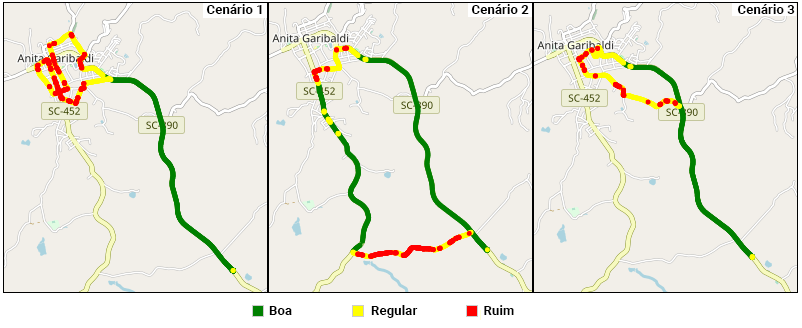
\includegraphics[width=1\textwidth]{figuras/fig_27.png}
   \fonte{Desenvolvido pelo autor.}
\end{figure}

\begin{table}[H]
\centering
\scriptsize
\caption{Quantificação para as classes de dados de qualidade de superfície} 
\label{table:qualidade_superficie_metricas}
\begin{tabular}{clccccccc}
\cmidrule(l){3-9} & & 
\multicolumn{4}{c}{\textbf{Número de Amostras}} & 
\multicolumn{3}{c}{\textbf{Distribuição das Classes de Dados (\%)}} 
\\ \midrule

\multicolumn{1}{c}{\textbf{Cenário}} &
\textbf{Conjunto} &
\textbf{Boa} &
\textbf{Regular} &
\textbf{Ruim} & 
\textbf{Total} &
\textbf{Boa} &
\textbf{Regular} &
\textbf{Ruim}
\\ \midrule

\multicolumn{1}{c}
{\multirow{8}{*}{1}} & PVS 1 Esquerda &  56577 & 65304 & 22155 & 144036 & 39,28 & 45,34 & 15,38 \\ \cmidrule(l){2-9} 
\multicolumn{1}{c}{} & PVS 1 Direita & 56595 & 66038 & 21403 & 144036 & 39,29 & 45,85 & 14,86 \\ \cmidrule(l){2-9} 
\multicolumn{1}{c}{} & PVS 4 Esquerda & 50744 & 62838 & 18910 & 132492 & 38,30 & 47,43 & 14,27 \\ \cmidrule(l){2-9} 
\multicolumn{1}{c}{} & PVS 4 Direita & 50732 & 64102 & 17658 & 132492 & 38,29 & 48,38 & 13,33 \\ \cmidrule(l){2-9} 
\multicolumn{1}{c}{} & PVS 7 Esquerda & 49855 & 64743 & 13950 & 128548 & 38,78 & 50,36 & 10,85 \\ \cmidrule(l){2-9} 
\multicolumn{1}{c}{} & PVS 7 Direita & 50040 & 67230 & 11278 & 128548 & 38,93 & 52,30 & 8,77 \\ \midrule

\multicolumn{1}{c}
{\multirow{8}{*}{2}} & PVS 2 Esquerda & 56086 & 37921 & 30677 & 124684 & 44,98 & 30,41 & 24,60 \\ \cmidrule(l){2-9} 
\multicolumn{1}{c}{} & PVS 2 Direita & 55926 & 38057 & 30701 & 124684 & 44,85 & 30,52 & 24,62 \\ \cmidrule(l){2-9} 
\multicolumn{1}{c}{} & PVS 5 Esquerda & 53715 & 32999 & 47163 & 133877 & 40,12 & 24,65 & 35,23 \\ \cmidrule(l){2-9} 
\multicolumn{1}{c}{} & PVS 5 Direita & 53510 & 32587 & 47780 & 133877 & 39,97 & 24,34 & 35,69 \\ \cmidrule(l){2-9} 
\multicolumn{1}{c}{} & PVS 8 Esquerda & 56466 & 29949 & 37203 & 123618 & 45,68 & 24,23 & 30,10 \\ \cmidrule(l){2-9} 
\multicolumn{1}{c}{} & PVS 8 Direita & 56617 & 32301 & 34700 & 123618 & 45,80 & 26,13 & 28,07 \\ \midrule

\multicolumn{1}{c}
{\multirow{8}{*}{3}} & PVS 3 Esquerda & 50923 & 46638 & 8255 & 105816 & 48,12 & 44,07 & 7,80 \\ \cmidrule(l){2-9}
\multicolumn{1}{c}{} & PVS 3 Direita & 50906 & 47384 & 7526 & 105816 & 48,11 & 44,78 & 7,11 \\ \cmidrule(l){2-9} 
\multicolumn{1}{c}{} & PVS 6 Esquerda & 40446 & 51051 & 4782 & 96279 & 42,01 & 53,02 & 4,97 \\ \cmidrule(l){2-9} 
\multicolumn{1}{c}{} & PVS 6 Direita & 40453 & 50180 & 5646 & 96279 & 42,02 & 52,12 & 5,86 \\ \cmidrule(l){2-9} 
\multicolumn{1}{c}{} & PVS 9 Esquerda & 42557 & 38919 & 10079 & 91555 & 46,48 & 42,51 & 11,01 \\ \cmidrule(l){2-9} 
\multicolumn{1}{c}{} & PVS 9 Direita & 42711 & 42625 & 6219 & 91555 & 46,65 & 46,56 & 6,79 \\ \bottomrule

\end{tabular}
\fonte{Desenvolvido pelo autor,}
\end{table}
